\documentclass[a4paper]{article}
\usepackage[margin=1.25in]{geometry}
\usepackage{amsmath}
\usepackage{ragged2e}
\usepackage[table,xcdraw]{xcolor}
\title{Atomic Spectra}
\date{March 19, 2018}
\author{Pablo Sevilla}
\usepackage{graphicx} 
\usepackage{float}
\usepackage{subcaption}



\begin{document}
  \pagenumbering{gobble}
  \maketitle
  \pagenumbering{arabic}
  
\begin{center}
  \section*{Abstract}
  \centering
  The spacing of the lines in a diffraction grating was found by examining the angles of the spectral lines produced by a helium lamp. With this information, the wavelengths of the spectrum produced by a hydrogen lamp were found. This allowed for the Rydberg constant to be calculated experimentally. The comparison between a helium-neon laser and a neon lamp's spectrum was analyzed, as well as to the spectrum of a helium lamp. We determined the grating constant $d$ to be $3.37973\times 10^{-6}$ millimeters. We experimentally determined the Rydberg constant and found it to be $10949005.71m^{-1}$, with an discrepancy of $0.23$ per cent compared to the literature value.
\end{center}
\newpage

\section{Introduction}
Electromagnetic radiation from the light source of a single element contains specific wavelengths. Some of these are in the visible spectrum, resulting in a unique visible signature to the human eye. When this collection of wavelengths hits a prism or a diffraction grating, the individual wavelengths get diffracted by different amounts. Each element has an intrinsic and unique spectrum. The study of this phenomenon is called spectroscopy, using such information to determine the chemicals present in any object, even intergalactic stars.
\subsection{Helium}
By using a diffraction grating that was perpendicular to the incident beam emitted from a helium lamp, the beam of the incident light is diffracted into certain angles, each depending on its wavelength. The relationship between the angle and wavelength when the incident beam passes through the diffraction grating is given by $m\lambda = d(sin(\theta_1) + sin(\phi))$ and $m\lambda = d(sin(\theta_2) - sin(\phi))$, where $\theta_1$ and $\theta_2$ are the angles of diffraction, $\lambda$ is the wavelength, $m$ is the order, $d$ is the grating constant, and $\phi$ is the angle the light will be incident on the grating. However, if we call the angles $\alpha_1$, $\alpha_2$, $\alpha_0$, where  $\alpha_0$ is the angle the light will be incident on the grating, then the angles of diffraction is measured by $\theta_1 = |\alpha_1 -\alpha_0|$ and $\theta_2 = |\alpha_2 -\alpha_0|$. Knowing this, we may define $\theta = \frac{1}{2}(\theta_1 + \theta_2)$ and $\Delta = \frac{1}{2}(\theta_1-\theta_2)$. Then $m\lambda = d(sin(\theta)(cos(\Delta))$. If $\Delta$ is small enough, to within a fraction of a degree, we may neglect $cos(\Delta)$ since , by a Taylor expansion, $cos(\Delta)$ will be approximately one. In this experiment, we will determine the grating constant $d$ by using the equation $d = \frac{m\lambda}{sin(\theta)cos(\Delta)}$, or $d =\frac{m \lambda}{sin(\theta)}$, if our $\Delta$ is small enough.
\begin{figure}[h]
\centering
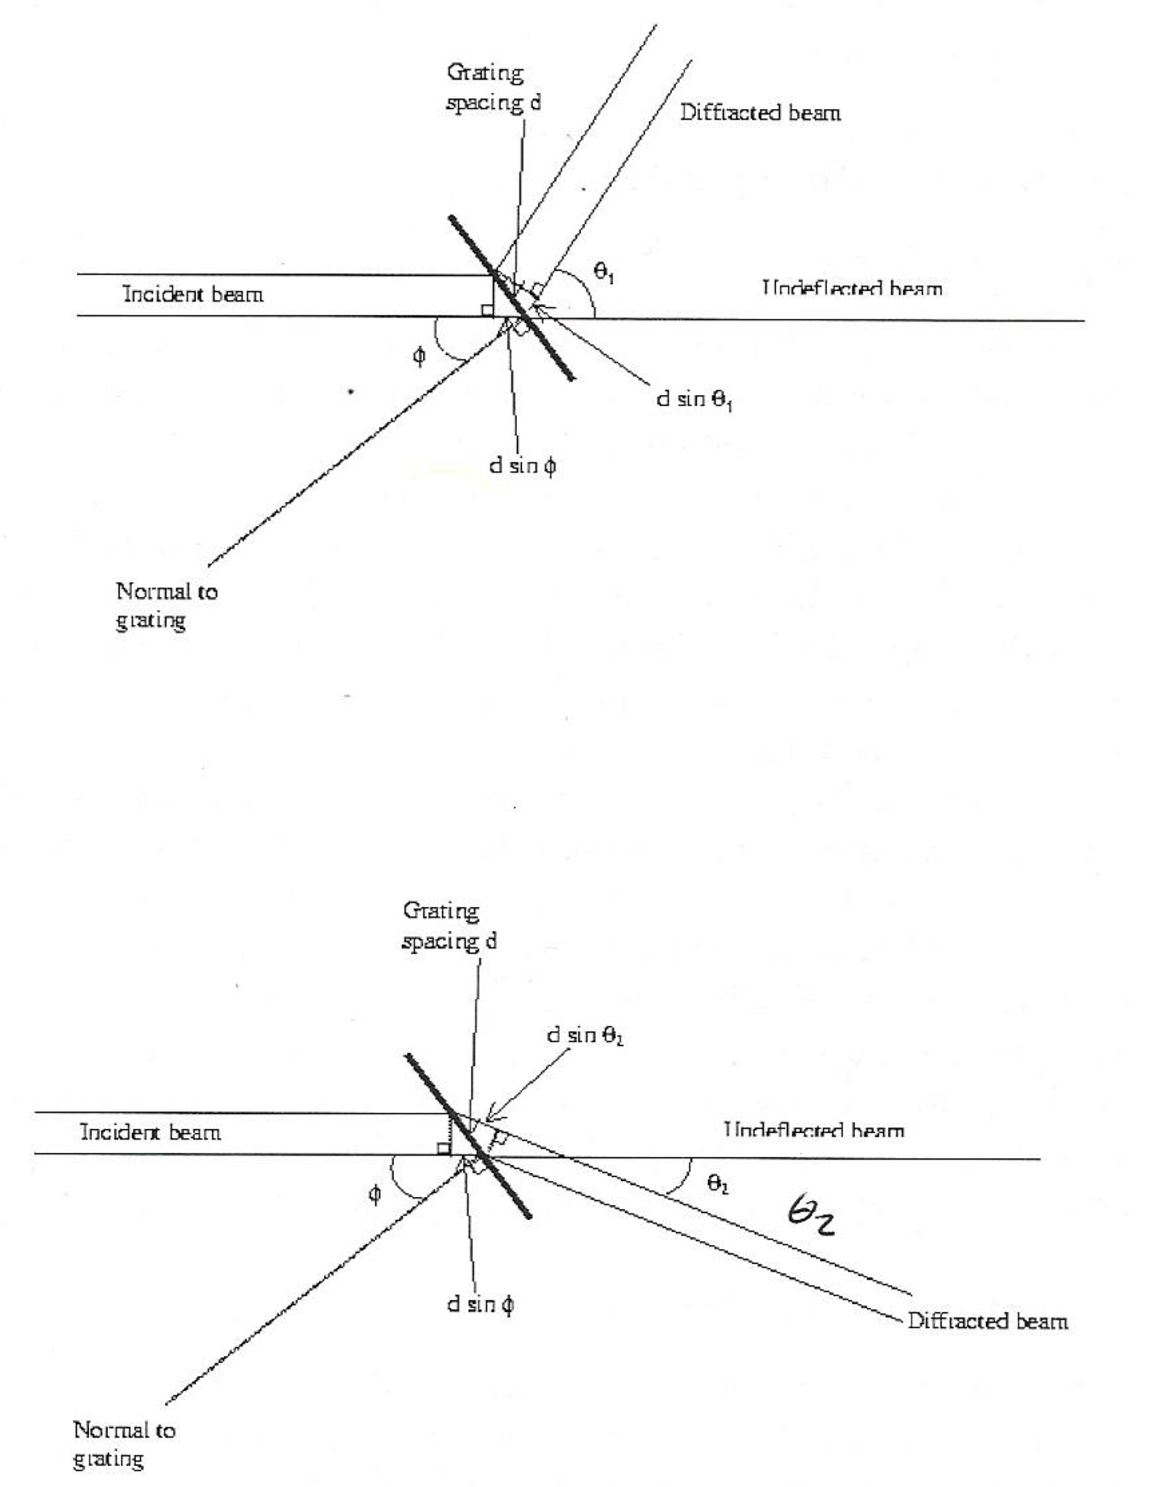
\includegraphics[width=0.5\textwidth]{1}
\caption{This figure shows an incident beam of light hitting a diffraction grating at an angle $phi$,which is normal to the diffraction grating, and refracted at two angles $\theta_1$ and $\theta_2$. However, the incident angle $\phi$ is the same as our measured incident angle $\alpha_0$. The angles $\theta_1$ and $\theta_2$ is the same as our measured angles $\alpha_1$ and $\alpha_2$, respectively. However, for this experiment, we made the incident angle $\alpha_0$,or $\phi$, as small as possible. This results in the incident beam being perpendicular to the diffraction grating  (Figure taken from Physics 133 lab manual at UC Santa Cruz)}
\end{figure}
\subsection{Hydrogen and Rydberg Constant}
By using the same diffraction grating that was used in the experiment involved with the helium lamp, the light emitted from a hydrogen lamp will also be distracted at certain angels, each depending on its wavelength (seen in figure 1). When an electron in an atom transfers from a higher energy state to a lower energy state $\Delta E$, a photon is released with the same change in energy $\Delta E$. Since the energy of a photon is related to its related to its wavelength, $\Delta E = \frac{hc}{\lambda}$ , each energy transition will have a unique wavelength that will be emitted, where $h$ is Planck’s constant, $c$ is the speed of light, and $\lambda$ is the wavelength. The quantum theory of the hydrogen atom describes the energy levels as $E_n = − \frac{\mu e^4}{8\epsilon_0 ^2h^2}\frac{1}{n^2}$ , where $\mu$ is the reduced mass $\frac{1}{\mu} = \frac{1}{m}+\frac{1}{M}$, where $m$ is the mass of the electron and $M$ is the mass of the proton, $\epsilon$ is the permittivity of free space, $e$ is the electron charge, and $n$ is a positive integer called the principal quantum number. The lowest energy state is $n = 1$, and as $n$ increases, the electron becomes further from the proton, with the separation increasing as $n^2$. Therefore the change in energy of a hydrogen atom is given by $\frac{\Delta E}{hc} = \frac{En_1−En_2}{hc} = \frac{\mu \epsilon^4}{8\epsilon_0 ^2h^3 c}(\frac{1}{n_2 ^2}-\frac{1}{n_1 ^2})$, where the constants $\frac{\mu e^4}{8\epsilon_0 ^2h^3 c}$ is known as Rydberg's constant $R_H$. Since we know that $\Delta E = \frac{hc}{\lambda}$ , we can say that $\frac{1}{\lambda} = \frac{\Delta E}{hc}$ , and thus $\frac{1}{\lambda} = (R_H)( \frac{1}{n_2 ^2}-\frac{1}{n_1 ^2} )$. In this experiment, we will determine the wavelengths of the diffracted light of the hydrogen spectrum by measuring the angles at which they are refracted and with the known grating constant $d$. With knowing those values for the wavelength, we will experimentally calculate the Rydberg constant $R_H$.

\subsection{Helium-Neon Laser}
When you create a potential difference in a helium-neon laser, the helium atoms will get excited. The energy of an excited helium atom may transfer its energy to a neon atom, which now puts the neon atom into an exited state and able to emit a photon. These photon emissions of a helium-neon laser happen at three wavelengths. Two of the wavelength are in the infrared spectrum, at 3.39 microns and 1.15 microns, while one wavelength occurs in the visible spectrum at 6328 Angstroms, which is a red light. Since we are unable to see the two wavelengths in the infrared spectrum, the visible wavelength will be of importance. In this experiment, we compare the visible 6328 Angstrom red light of the helium-neon laser to the spectrum of a neon lamp and to the spectrum of a helium lamp.

\section{Procedure}
\subsection*{Apparatus}
\begin{itemize}
  \item \textbf{Diffraction Grating} - A piece of glass with many parallel lines where light cannot pass through.
  \item \textbf{Spencer Spectrometer} - Device used to calculate the angle to which spectral lines are diffracted to. Contains a very sensitive vernier scale, objective lenses, telescope, an eyepiece and screws to carefully change the angle.
  \item \textbf{Laser} - Helium-Neon Laser of a power of $0.78mW$.
  \item \textbf{Helium Lamp} - A lamp with only helium inside. When current is passed through it, excitations occur and spectral lines are emitted.
  \item \textbf{Hydrogen Lamp} - Another lamp but using hydrogen inside it.
\end{itemize}
\subsection{Alignment of the Spencer Spectrometer}
A Spencer Spectrometer was used to view and measure the light spectrum of the lamps used (see figure 2). In order to obtain accurate measurements, the Spencer Spectrometer must be properly aligned. First, the cross-hairs in the telescope were brought to focus. The helium lamp was then placed in the power source, so that the helium lamp will start to emit photons whenever there is a voltage applied to it. The lamp was put behind the entrance slit of the collimator, which guided the light emitted from the lamp to the diffraction grating (which is not in the grating hold yet). The lamp must be placed directly in front of the slit so that as much light as possible may pass through the slit. Furthermore, the telescope was rotated so that was it was nearly parallel to the collimator, with the light emitted from the helium lamp visible while peering through the eyepiece of the telescope. This light will look like a vertical line resembling the same color as the light emitted from helium lamp. The helium lamp needs to be in focus and not blurry, so we focused both the collimator and the telescope in order to achieve this. Also, the slit width must be as small as possible so that more accurate measurements are taken, while keeping in mind that enough light needs to go through the entrance slit of the collimator so that the emitted light will be visible. If the slit width is too small, not enough light will get through and the spectrum lines will be too dim to see. If the slit width is too large, the spectrum lines will be too large to get an accurate measurement of the angle. Subsequently, the cross-hairs in the telescope must be in the middle of the light that was passing through the collimators entrance slit. This means that the collimator and the telescope are parallel to each other.

After the collimator and the telescope are parallel to each other with the emitted light from the helium lamp is focused, we needed to get the diffraction grating perpendicular to the collimator. This will, in turn, also be perpendicular to the telescope, since the telescope is parallel to the collimator. To do this, a mirror was placed in the diffraction grating slot and a battery was attached to the telescope, which cast a shadow of the cross-hairs on the mirror. The grating table was then leveled and rotated with the adjustment screws on the grating table until the shadow of the cross-hairs was superimposed on the actual cross-hairs. This means that the mirror, or soon-to-be diffraction grating, is now perpendicular to the telescope and collimator. The mirror was replaced with the diffraction grating and the cross-hairs was focused on the undeflected light.

The vernier scale on the Spencer Spectrometer was calibrated so that it measured zero degrees. However, this would create a challenge with reading the vernier scare. To make the readings easier, we set our zero mark to $90°+2'$. When we measured this angle, which is our $\alpha_0$, it came to be $90$,. Since the diffraction grating is nearly perpendicular to the incident light beam, the light will be refracted left and right at almost the same angles. If these angles are not close to each other, then the Spencer Spectrometer is not properly aligned. Repeat the process of alignment until these angles have nearly the same value.
\begin{figure}[h]
\centering
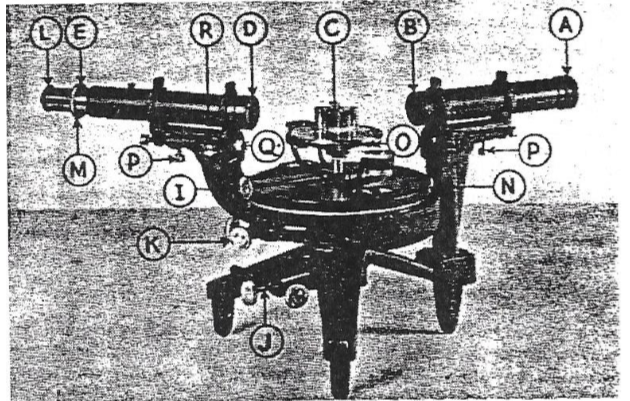
\includegraphics[width=0.5\textwidth]{2}
\caption{This figure shows a model of a Spencer Spectrometer. A: The slit where the light emitted from a lamp enters; B: The objective lens of the collimator; C: This is the diffraction grating; D: The objective lens of the telescope; E: This is where the cross-hairs are located in the telescope; L: This is where the eyepiece of the telescope is located; O: This is where the grating table leveling screws are located; I: This is the screw that is used to lock the telescope into place so that it will not move if pushed or hit. Since the Spencer Spectrometer is not exactly like the one shown here, the remaining points in the figure are not important. (Figure taken from Physics 133 lab manual at UC Santa Cruz)}
\end{figure}

\subsection{Helium}
The helium lamp has a known spectrum, which means that we know the wavelengths of the spectral lines helium. We do not know the grating constant d of the diffraction grating this is used. By measuring the angles of the spectral lines of helium, $\alpha_1$ and $\alpha_2$, and knowing the wavelengths of helium's spectrum, we are able to find the grating constant $d$. Since we know the incident angle of the beam of light $\alpha_0$, we may find the angles $\theta_1$ and $\theta_2$ by $\theta_1 = |\alpha_1 − \alpha_0|$ and $\theta_2 = |]\alpha_2 −\alpha_2|$, respectively. Since the beam of light is not perfectly perpendicular on the diffraction grating, the diffraction angle of the spectrum will not be exactly the same on each side of $\alpha_0$, but will be approximately the same if the Spencer Spectrometer is properly aligned. By the theory of diffraction gratings, $\theta$ and $\Delta$ are found by $\theta = \frac{1}{2}(\theta_1 + \theta_2)$ and $\Delta = \frac{1}{2}(\theta_1 −\theta_2)$. Then the grating constant d may be calculated by $d = \frac{m\lambda}{sin(\theta)cos(\Delta)}$, where $m$ is the order of the spectrum and $\lambda$ is the wavelength, which is found in the table in the appendix. Although a Spencer Spectrometer that is perfectly aligned will have a $\Delta$ equal to zero, by the Taylor expansion of $cos(x)$, if $\Delta$ is small enough, $cos(\theta)$ will approximately be one. Therefore you may omit the $cos(\Delta)$ and the grating constant d may be determined by $d = \frac{m\lambda}{sin(\theta)}$. Each measured spectral line of helium will correspond to a grating constant $d$. Since there will be error in the measurements, it is needed to propagate the error through the calculations to show that the error carries through the equations and effects the final results. Also, the weighted mean of the grating constant must be found, since there are multiple measurements of the grating constant $d$.
\subsection{Hydrogen}
With the average grating constant known, the hydrogen spectral lines may be measured and calculated. This is be done by taking the equation used to find the grating constant and using algebra to solve for the wavelength $\lambda$, which turns out to be $\lambda = \frac{dsin(\theta)cos(\Delta)}{m}$ . If $\Delta$ is small enough, $cos(\Delta) ≈ 1$, so then $\lambda = \frac{dsin(\theta)}{m}$ . While viewing the hydrogen spectrum, we made sure to only measure the Balmer series. The hydrogen lamp may emit a few spectral lines that do not correspond to the Balmer series, which are emitted by molecular hydrogen.
\subsection{Determine the Rydberg Constant}
With the wavelengths of the hydrogen spectrum now known, we were able to experimentally calculate the Rydberg Constant $R_H$. The wavelengths of the spectral lines of hydrogen is related to the Rydberg constant by the equation $\frac{1}{\lambda}  = R_H( \frac{1}{n_2 ^2}-\frac{1}{n_1 ^2} )$. Since we want to calculate the Rydberg constant, by doing algebra to the equation above, $R_H = \frac{1}{\lambda}\frac{1}{( \frac{1}{n_2 ^2}-\frac{1}{n_1 ^2})}$. Each of the hydrogen spectrum lines will result in a calculated value for the Rydberg constant, so the weighted mean of the calculated values will be used as the experimentally determined Rydberg constant.
\subsection{Helium-Neon Laser}
In order to compare the neon lamp with the helium-neon laser, we placed a piece of cardboard in front of the bottom half of the collimator’s entrance slit. This will obstruct some of the neon lamp's light resulting in neon's spectrum to show in the bottom half of the telescope's eyepiece. We then aimed the helium-neon laser so that the laser dot is on the cardboard in front of the collimator’s entrance slit. This will scatter the emitted light into the collimator (see figure 3). This will result in the neon's spectrum to show in the bottom half of the telescope's eyepiece, while the spectrum of the helium-neon laser will show in the upper half of the telescope's eyepiece. The spectrum of the helium-neon laser will be one visible line of light, while the spectrum of neon will have many visible lines of light. Compare these two spectra with the eye and take measurements of the angles. We repeated this process with the helium lamp.
\begin{figure}[h]
\centering
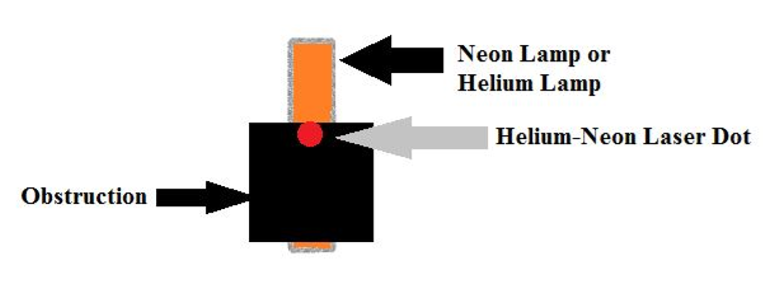
\includegraphics[width=0.5\textwidth]{3}
\caption{This figure shows what the set up of the helium-neon laser and the neon lamp, or helium lamp, should look like. Place the cardboard, or any material that will obstruct the light emitted from the neon, or helium, lamp. Aim the helium-neon laser dot on the obstruction and in front of the collimator’s entrance slit so that the emitted light will scatter into the collimator’s entrance slit.}
\end{figure}
\section{Data and Analysis}
\subsection{Helium and Grating Constant}
Before we took measurements, we looked to see how many spectral lines of the helium lamp that were visible and, we saw eight spectral lines. We measured our incident beam angle $\alpha_0$ to be $90°+2'$ The measurements of the angles of the spectral lines of helium are shown in table 1. Each of the measured angles, $\alpha_1$ and $\alpha_2$, were not the exact same value, as seen by the $\theta_1$ and $\theta_2$ values. This is due to an error in measurement from reading the vernier scale on the Spencer Spectrometer and from the cross-hairs not being exactly in the middle of the light from the helium spectrum, and that our Spencer Spectrometer was not perfectly aligned. However,by the Taylor expansion of $cos(x)$, the measurements result in $cos(\Delta)$ being close enough to one that $cos(\Delta)$ may be ignored in calculations. Also, all of the values in table 1 are in degrees, so they were converted into radians for the calculations by multiplying the value of degrees by $\frac{\pi}{180}$.

Using the values for $\theta$ in table 1 and the known wavelengths of the helium spectrum, we calculated the grating constants $d$. By using $\frac{1}{d} = \frac{sin(\theta)}{m\lambda}$, we also calculated the lines per millimeter for the diffraction grating. These values are shown in table 2. Since there are multiple values for both $d$ and $\frac{1}{d}$, a weighted mean was calculated. We obtained the following results (see next page):
\begin{figure}[h]
\centering
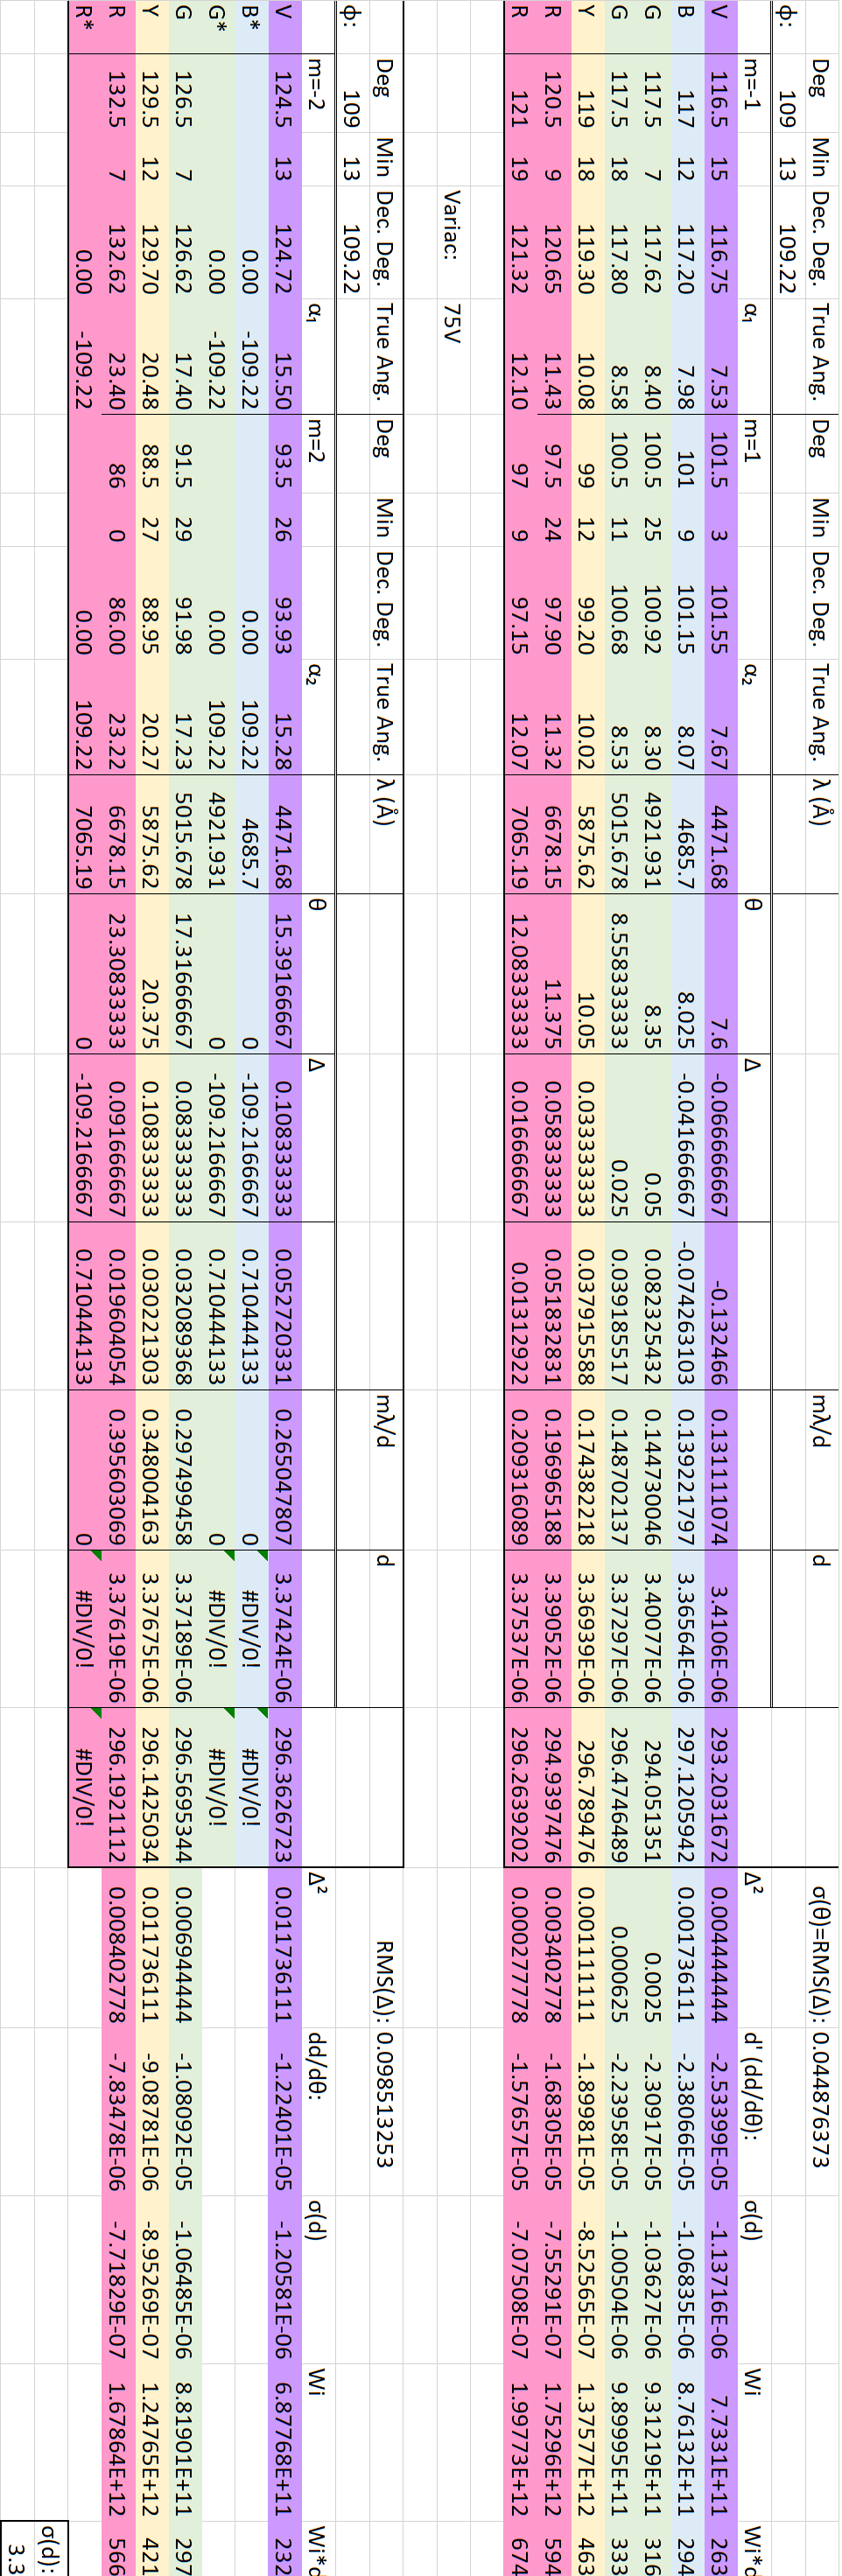
\includegraphics[width=0.5\textwidth]{he1}
\end{figure}
\clearpage
\begin{figure}[h]
\centering
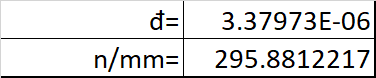
\includegraphics[width=0.5\textwidth]{he2}
\end{figure}

\subsection{Hydrogen}
The recorded angles for the hydrogen spectrum are shown in the table below. Our recorded data was measured in degrees. The data shown in the table was converted from degrees to radians for the calculations by multiplying the value of degrees by $\frac{\pi}{180}$. Again, our $\Delta$ calculations are small enough to omit $cos(\Delta)$ from our calculations. Since the grating constant $d$ is known, the wavelength of the lines found in the hydrogen spectrum were calculated by $\lambda = \frac{dsin(\theta)}{m}$.
\begin{figure}[h]
\centering
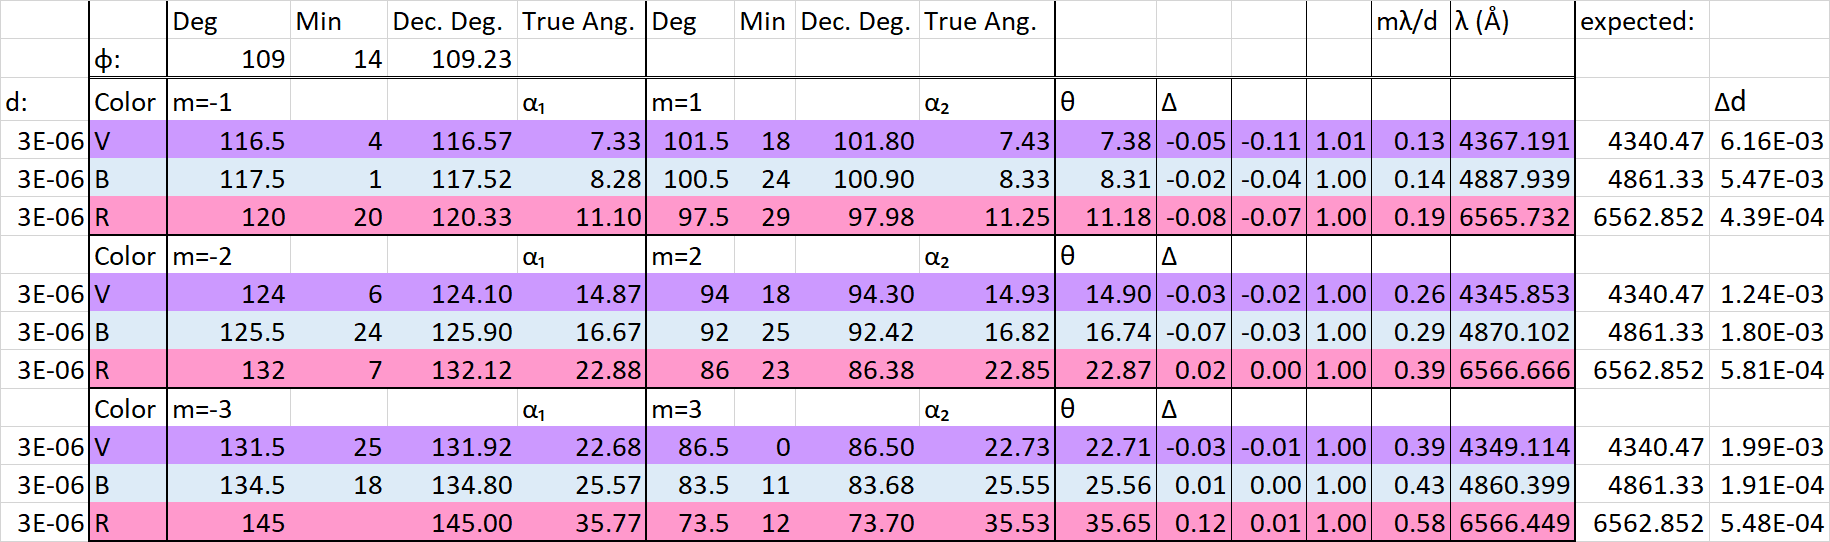
\includegraphics[width=1.15\textwidth]{hy1}
\end{figure}
\subsection{Calculating the Rydberg Constant}
The values for the Rydberg constant were calculated from each wavelength found for the spectral lines of the hydrogen lamp by the equation $R_H = \frac{1}{\lambda} \frac{1}{(\frac{1}{n_2 ^2}-\frac{1}{n_1 ^2})}$. The values of the calculated Rydberg constant and their weighted mean are shown below:
\begin{figure}[h]
\centering
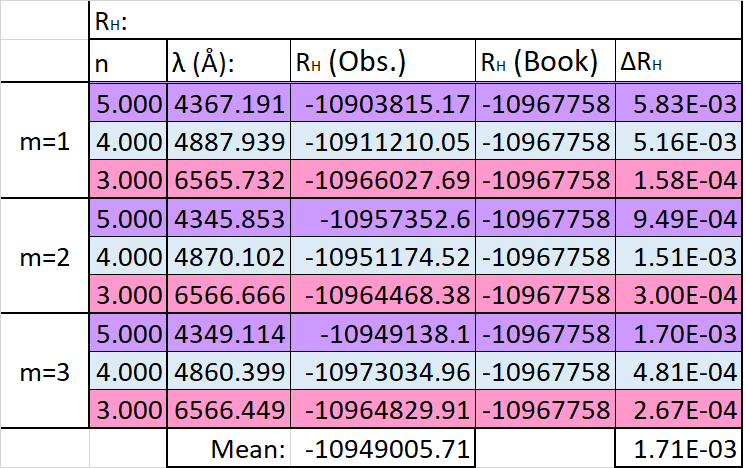
\includegraphics[width=0.5\textwidth]{hy2}
\end{figure}

Our experimental value of the Rydberg constant is consistent with the literature value by a factor of $0.23$ per cent.
\clearpage
\subsection{Helium-Neon Laser}
The spectrum of the neon lamp contained many lines - mainly of red, orange and green - that were very close to each other. When the spectrum produced by the laser was compared to the spectrum emitted by the neon lamp, only one line from the neon spectrum aligned with the spectrum of the laser. The color of the aligned lines was red. When we measured the angles of the lines of both spectra that were aligned, it was found that both resulted in the same angle.
\begin{figure}[h]
\centering
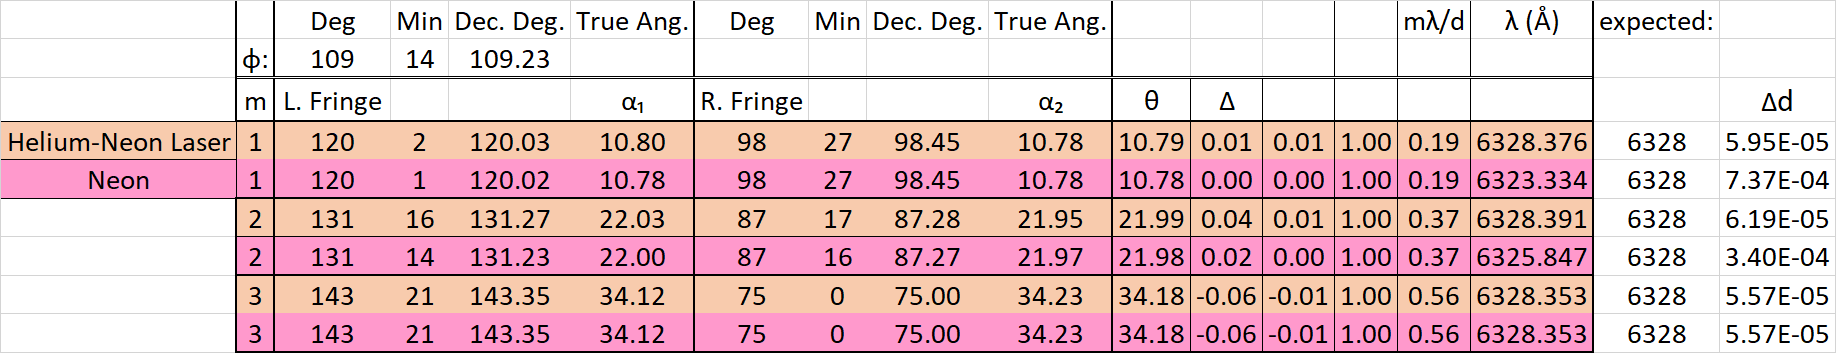
\includegraphics[width=1.0\textwidth]{laser}
\end{figure}
Since the measurements are in degrees, we had to convert them to radians by multiplying the values of degrees by $\frac{\pi}{180}$. The grating constant $d$ is already known to be $3.37973\times 10^{-6}$. We then calculated the wavelength of the line produced from the helium-neon laser, as well as the line from the spectrum of the neon lamp that it aligns with, by using the equation $\lambda = \frac{dsin(\theta)}{m}$. The neon lamp was then replaced with the helium lamp, while the orientation with the laser was maintained. When the spectrum produced by the helium lamp was compared to the spectrum emitted by the helium-neon laser, it was found that no lines from each spectrum aligned with each other. The spectra do not align since it is the neon atoms in the helium-neon laser that emit the photons. Thus, the spectrum of the helium-neon laser is aligned with one of the lines produced by the spectrum of the neon lamp, which confirms that it is indeed the neon atoms that are emitting photons and not the helium atoms.

\section{Conclusion}
From using a helium lamp with the wavelengths of the spectrum of helium known, we determined the grating constant $d$ to be $3.37973\times 10^{-6}$ millimeters. With the grating constant known, we were able to calculate the wavelengths of the spectrum that is emitted by the hydrogen lamp. Using the found wavelengths of the hydrogen spectrum, we experimentally determined the Rydberg constant and found it to be $10949005.71m^{-1}$. Since the grating constant of the diffraction grating is known, the wavelength of the spectrum of a helium-neon laser was able to be calculated. We compared the spectrum of the helium-neon laser to the spectrum emitted by a neon lamp and also by a helium lamp. The spectrum of the helium-neon laser matched a line of the spectrum of the neon lamp, while the helium-neon laser’s spectrum did not match up with any lines from the helium lamp.

\clearpage

\section{References}
\begin{itemize}
\item Physics 133 2018 Lab Manual at University of California Santa Cruz
\end{itemize}


\end{document}